\styledchapter{Auctions}

Why are economic theorists interested in auctions?

\begin{example}[Real-world auctions]
	There are several useful auctions used in everyday life:
	\begin{itemize}
		\item Art, used cars, etc.
		\item Electricity \faLightbulb
		\item Google/Facebook ads
		\item Electromagnetic spectrum
		\item Government debt
	\end{itemize}
\end{example}

We start with a simple example.

\section{Optimal Posted Price With a Single Buyer}

Suppose we have a single buyer for a single good, with the buyer's value as $v \in [0,\overline{v}]$. 
Let $v \sim F$, where $\P\left[v \le w\right] = F(w)$.
\begin{assumption}
	We assume $F$ is differentiable and thus admits a density $f$. We further assume that the seller has no value for the good.
\end{assumption}

\begin{proposition} \label{4-22-3}
	In this single-buyer, single-good environment with a posted price, the optimal price is the $p^\star$ satisfying \[
		p^\star = \frac{1-F(p^\star)}{f(p^\star)}
	.\] 
	\begin{itemize}
		\item The optimal price leads to an inefficient outcome, and
		\item The optimal price depends on $F$.
	\end{itemize}
\end{proposition}
\begin{proof}
	With price $p$, the seller's expected revenue is \[
		p \underbrace{(1- F(p))}_{\mathclap{\text{probability the buyer buys}}}
	.\] 
	The first order condition is \[
		1-F(p) + p\left( -f(p) \right) = 0
	,\] so the optimal posted price is \[
		p^\star = \frac{1-F(p^\star)}{f(p^\star)}
	.\] 
	Who is the lowest type that purchases the good? It is the person with value $v = p^\star$, yielding the \emph{virtual value} characterization: \[
		v - \frac{1-F(v)}{f(v)} = 0
	.\] 
	We see a source of inefficiency;\boxednote{For example, with a uniform value distribution $v \sim \operatorname{Unif}(0,1)$, the virtual value is negative for $v < 1 / 2$.} even though the seller has no value for the good, she does not sell the good to buyers with low types, even though post-revealing type, the sale could go through with a price between $0$ and the realized value to make everyone better off.
\end{proof}

\section{Overview of Auctions}

Consider a set $N$ of agents who are the possible buyers of the single good, where each agent $i $ has value $v_i \in [0,1]$. Let the set of outcomes be \[
	A = \left\{\left( x_1,\ldots,x_{\left| N \right|} \right): x_i \ge 0\  \forall i, \sum\limits_{i \in N}^{} x_i \le 1\right\}
.\] Hence, an outcome is a lottery over who gets the good (including the seller herself).

\begin{assumption}
	\boxednote{Since the agent has linear utility in money, it's equivalent to charge agent $i$ if she wins vs. charging a smaller amount proportional to her winning probability, regardless if she wins.}
	We assume the utilities take the following form: If agent $i$ has value $v_i$ for the good, gets it with probability $x_i$, and pays $p_i$, then the payoff is \[
		u_i = v_i x_i - p_i
	.\] 

	The price $p_i$ is determined by the reported value, which may not be the same as the true value.
\end{assumption}

\begin{example}[Common auctions]
	We have the following common auctions:
	\begin{enumerate}[label = (\roman*)]
		\item \textbf{First-price auction}: The seller asks each $i \in N$ to submit a bid $b_i \ge 0$. The player with the highest bid wins and pays their bid.
		\item \textbf{Second-price auction}: The player with the highest bid wins and pays the second highest bid.
		\item \textbf{All-pay auction}: The player with the highest bid wins and every player $i$ pays $b_i$.
	\end{enumerate}
\end{example}

We specialize to a two-player symmetric case.

\begin{assumption}
	Let $N = \left\{1,2\right\}$ and $v_i \overset{iid}{\sim} F$. Assume $F$ admits a density $f$ that is strictly positive on $[0,1]$ and $0$ elsewhere.
\end{assumption}

\begin{proposition}[Revenue of a second price auction]
	The revenue of a second-price auction is \[
		R_{\text{SPA}} = 1 - \int_{0}^{1} F_{(2)}(w)dw = \int_{0}^{1} \left( 1-F(w) \right)^2dw 
	.\] 
\end{proposition}

\begin{proof}
	We know that truthful reporting is a dominant strategy in a second-price auction. Assume that $b_i = v_i$ for both agents.
	To understand the expected revenue, we need to understand the distribution of the lower value.
	We see that \boxednote{We can take the derivative of $F_{(2)}$ to get \[
		f_{(2)}(w) = 2f(w) - 2F(w)f(w)
	.\] }\[
		F_{(2)}\left( w \right) = 1- (1-F(w))(1-F(w)) = 2F(w) - F(w)^2
	,\] as both players must have value \emph{above} $w$.
	Hence, the expected revenue is \[
		R = \int_{0}^{1} w f_{(2)}(w)dw = 1- \int_{0}^{1} F_{(2)}(w)dw 	
	,\] 
	where the second equality follows from integrating by parts.
\end{proof}

The first-price auction analysis is trickier --- we intuit that people should shade bids, so the effect of taking the highest bid may be offset by lower bids overall.
We need to first take a detour to Bayesian games, where agents are unsure of others' payoffs.

\begin{definition}[Bayesian game]
	A Bayesian game is defined by the following primitives:
	\begin{itemize}
		\item A set $N$ of agents.
		\item For each $i \in N$, there is a set of types $T_i$ which encodes her own type and her beliefs over others' types. We denote the type space $T \coloneqq \prod_{i \in N}^{} T_i $.
		\item For each $i \in N$, there is a set of actions $A_i$, and we denote the set of action profiles $A \coloneqq \prod_{i \in N}^{} A_i $.
		\item For each $i \in N$, there is a utility function \[
			U_i: T_i \times A \to \R
		.\] 
		\item (We assume there is) A common prior $\mu \in \Delta(T)$. Player $i$'s belief over the others' types is determined by conditioning $\mu$ on her realized type $t_i \in T_i$ and is notated $\mu\left( t_{-i} \mid t_i \right)$.
	\end{itemize}
	A strategy for player $i$ is a function \[
		\sigma_i : T_i \to \Delta(A_i)
	.\] The strategy profile $\sigma = \left( \sigma_i \right)_{i \in N}$ induces the payoff for agent $i$ \[
		U_i(\sigma, t_i) = \sum\limits_{t_{-i}} \sum\limits_{a \in A}^{} u_i(t_i,a) \sigma_i\left( a\mid t_i \right) \sigma\left( a_{-i} \mid t_{-i} \right) \mu\left( t_{-i}\mid t_i \right)
	.\] 
	The strategy profile $\sigma$ is a Bayes-Nash equilibrium if for every agent $i$, $\sigma$, $\sigma_i'$, and $t_i$, \[
		U_i\left( \sigma,t_i \right) \ge U_i\left( \left( \sigma_i', \sigma_{-i} \right), t_i \right)
	.\] 
\end{definition}

Now we are ready to analyze the first-price auction. \boxednote{Note that all the primitives of the Bayesian game map neatly onto our auction. The common prior $\mu \in \Delta(T)$ is the distribution from which the values are drawn from.}

\begin{proposition}[Revenue of a first-price auction]
	An equilibrium bidding strategy in a symmetric first price auction with independent value distribution with CDF $F$ for a bidder with value $v$ is \[
		b(v) = v - \frac{1}{F(v)} \int_{0}^{v} F(w)dw 
	.\] 
	The expected revenue is \[
		R_{\text{FPA}} = 1 - \int_{0}^{1} F_{(2)}(w)dw = \int_{0}^{1} \left( 1-F(w) \right)^2dw 
	,\] 
	which is exactly the expected revenue of the second-price auction.
\end{proposition}

\begin{proof}
	To prove the proposition, we begin with a conjecture that there is an equilibrium of the first-price auction in which there is a function $b: [0,1] \to [0,1]$ such that agent $i$ bids $b(v)$ when she has value $v$. We also conjecture that this $b$ is strictly increasing and differentiable.

	A necessary condition for a proposed $b$ to be a Bayes--Nash equilibrium is that when player $i$ has value $v_i$, her utility bidding according to $b(\cdot)$ is maximized when bidding as if she has value $v_i$:\footnote{The utility in this expression is the utility when both players bid according to $b(\cdot)$, player $j$ bids according to his true value, and player $i$ bids as if she had value $v_i'$.} \[
		v_i = \argmax_{v_i' \in [0,1]} \left( v_i - b(v_i') \right)F(v_i')
	.\]
	The first-order condition is \[
		-b'(v_1') F(v_1') + \left.\left( v_i - b(v_i') \right)f(v_i')\right|_{v_i' = v_i} = 0
		,\] which yields \boxednote[13\baselineskip]{When we divide by $F(v)$ in the last line, there is a problem if $v=0$; we can assume/show that an agent must bid $0$ if she has value $0$.}
	\begin{align*}
		b'(v_i) F(v_i) + b(v_i) f(v_i) &= v_i f(v_i) \\
		\frac{d}{dv_i} b(v_i) F(v_i) &= v_i f(v_i) \\
		\int_{0}^{v}  \frac{d}{dv_i} b(v_i) F(v_i) dv &= \int_{0}^{v}  v_i f(v_i) dv \\
		\left. b(v_i) F(v_i) \right|_{0}^{v} &= \int_{0}^{v} v_i f(v_i) dv_i \\
			b(v)F(v) &= \left. v_i F(v_i)\right|_{0}^{v} - \int_{0}^{v} F(v_i) dv_i \\
				b(v)F(v) &= vF(v) - \int_{0}^{v} F(v_i) dv_i \\
				b(v) &= v - \frac{1}{F(v)}\int_{0}^{v} F(w)dw 
	.\end{align*}
	For later use, we compute that \[
		b'(v) = 1 + \frac{f(v)}{F(v)^2} \int_{0}^{v} F(w)dw - \frac{1}{F(v)}F(v) = \frac{f(v)}{F\left( v \right)^2} \int_{0}^{v} F(w)dw  
	.\] 

	If the conjectured restrictions on the equilibrium hold, then we have one candidate function.
	By the assumption that $b$ is increasing, expected revenue depends on the distribution of the higher value, which we find to be characterized by 
	\begin{align*}
		F_{(1)}(w) = F(w)^2, \quad f_{(1)}(w) = 2F(w)f(w)
	.\end{align*}
	Hence, expected revenue is
	\begin{align*}
		R_{\text{FPA}}
		&= \int_{0}^{1} b(w) f_{(1)}(w)dw  \\
		&= \left. b(w) F_{(1)}(w) \right|_0^{1} - \int_{0}^{1} b'(w) F_{(1)}(w)dw \\
		&= b(1) - \int_{0}^{1} \frac{f(w)}{F(w)^2}\left( \int_{0}^{w} F(z)dz  \right)\underbrace{F_{(1)}(w)}_{\smash{=F(w)^2}}dw \\
		&= \overbrace{1-\int_{0}^{1} F(w)dw }^{\smash{b\left(1 \right)}} - \int_{0}^{1} f(w) \left( \int_{0}^{w} F(z)dz  \right)dw \\
		&= 1 - \int_{0}^{1} F(w)dw - \left[ F(v) \int_{0}^{1} F(w)dw  \right]_{v=0}^{v=1} + \int_{0}^{1} F\left( v \right)^2 \\
		&= 1- 2 \int_{0}^{1} F(w)dw + \int_{0}^{1} F(w)^2dw \\
		&=  1 - \int_{0}^{1} F_{(2)}(w)dw = R_{\text{SPA}}
	.\end{align*}
\end{proof}

\section{Revelation Principle}

The Revelation Principle greatly simplifies analysis of equilibria of games.

\begin{definition}[Direct mechanism]
	A direct mechanism is a game where $\mathscr{A}_i = V$ so that agents report a value $v$.
\end{definition}

\begin{proposition}[Revelation Principle]
	For any $G$ and equilibrium $s$, there exists a direct mechanism in which it is a Bayes--Nash equilibrium for agents to truthfully report such that the outcome (set of allocation probabilities and transfer payments) is the same under $G, s$ and under the direct mechanism.
\end{proposition}

\begin{proof}
	Let $G \coloneqq \left( \left( \mathscr{A}_i \right)_{i \in N},x,p \right)$, fix an equilibrium strategy profile $s \coloneqq \left( s_i \right)_{i \in N}$. 

	Consider the direct mechanism $M \coloneqq \left( \left( V \right)_{i \in N}, x',p' \right)$ with
	\begin{align*}
		x'(v_1,\ldots,v_{\left| N \right|}) &= x\left( s_1(v_1),\ldots,s_{\left| N \right|}\left( v_{\left| N \right|} \right) \right) \\
		p'(v_1,\ldots,v_{\left| N \right|}) &= p\left( s_1(v_1),\ldots,s_{\left| N \right|}\left( v_{\left| N \right|} \right) \right)
	.\end{align*}
	Then $M$ has an equilibrium in which all agents truthfully report --- a unilateral deviation corresponds to misplaying $s_i(v_i)$ as $s_i(v_i')$ in $G$, which was shown to not be optimal.\boxednote{In the direct mechanism, a unilateral deviation is just a different report $v_i'$, which induces the original-game action $s_i(v_i')$. The revelation principle does not compare against arbitrary alternative strategies $s_i'$ in the direct mechanism; those deviations were already covered by the assumption that $s$ is an equilibrium of the original game.}
\end{proof}

\section{Revenue-Maximizing Auctions}

Consider a seller who wants to design a game\boxednote{We only consider the strategic-normal form.} $G$ to maximize revenue with the following structure. For each $i \in N$, there is an action set $\mathscr{A}_i$. We denote the action profile $\mathscr{A} \coloneqq \prod_{i \in N}^{} \mathscr{A}_i $. 
The components of the game the seller must design are \boxednote{Here, just think of $\mathscr{A}_i \coloneqq V_i = [0,1]$ as the possible set of values for agent $i$ to report. This is because we can appeal to the Revelation Principle, which follows in two paragraphs.}
\begin{align*}
	&x: \mathscr{A} \to A \\
	&p: \mathscr{A} \to \R^{\left| N \right|}
.\end{align*}

Each agent $i \in N$ comes up with a strategy $s_i : V \to \Delta \mathscr{A}_i$. Note that we are still assuming agent $i$ has value $v_i \overset{iid}{\sim} F$ in $[0,1]$. Assume the profile $s\coloneqq \left( s_i \right)_{i \in N}$ is a Bayes--Nash equilibrium of the game $G$.

By the Revelation Principle, for any equilibrium of an auction, there exists a direct mechanism with truthful reporting as a Bayes--Nash equilibrium such that the allocation probabilities and payments are the same under the two mechanisms.
In particular, the expected revenues will be equal, so when trying to determine the maximum achievable revenue, it suffices to consider the maximum attainable revenue under truth-telling direct mechanisms; we can safely assume that the reported value $s_i$ is exactly $v_i$.

Fixing $\left( s_i \right)_{i \in N} = \left( v_i \right)_{i \in N}$, let's focus on one agent $i$ and drop subscripts.
Let $i$'s interim allocation $X(v)$ be the probability that $i$ gets the good when she reports value $v$.\boxednote{Capital $X$ and $P$ denote expectations of win probabilities and payments when an agent knows her value but not those of others. We call them \emph{interim} functions because they are not ex-ante (before an individual learns her own value) nor ex-post (after an individual learns everyone's values).} Let $P(v)$ be $i$'s expected payment when she reports value $v$.
In this case, $i$'s expected utility is $vX(v) - P(v)$, so under our assumption of $\left( s_i \right)_{i \in N} = \left( v_i \right)_{i \in N}$ being an equilibrium,
\begin{align*}
	vX(v) - P(v) &\ge vX(v') - P(v') \\
	v'X(v') - P(v') &\ge v' X(v) - P(v)
.\end{align*}
for every potential misreport $v' \in V \coloneqq [0,1]$.
Rearranging, these lead to 
\begin{align*}
	v\left( X(v) - X(v') \right) &\ge P(v) - P(v') \\
	v'\left( X(v') - X(v) \right) &\ge P(v') - P(v) \\
	\iff v'\left( X(v) - X(v') \right) &\le P(v) - P(v')
,\end{align*}
which imply the \emph{payment difference sandwich}:
\begin{equation}
	v'(X(v) - X(v')) \le P(v) - P(v') \le v\left( X(v) - X(v') \right) \label{4-20-a}
\end{equation}
We will derive several properties from Equation (\ref{4-20-a}).

We first characterize the interim assignment probabilities and payments of a Bayes--Nash equilibrium. \boxednote{Thinking ahead, if we're hoping to find probability assignments and a payment structure that is revenue-maximizing in an equilibrium, it must at least satisfy these conditions. Corollary (\ref{4-20-c}) adds a further restriction for when we specialize to an individually-rational auction that is actually revenue-maximizing.} These are \emph{necessary} conditions for \emph{all} equilibria of auctions, and not just revenue-maximizing ones (though these are really the ones we care about the most).

\begin{proposition} \label{4-20-b}
	If $s$ is a Bayes--Nash equilibrium of an auction game $G$, then the induced interim allocation probabilities $X_i$ and payments $P_i$ satisfy the following:
	\begin{enumerate}[label = (\roman*)]
		\item The interim allocation probability $X(\cdot)$ is nondecreasing in the report.
		\item For any $v$, \[
			P(v) = P(0) + vX(v) - \int_{0}^{v} X(t)dt 
		.\] The only choices that the seller has are in controlling $P(0)$ and $X(v)$ for each $v \in [0,1]$. The payment at any value is then uniquely determined.
	\end{enumerate}
\end{proposition}

\begin{proof}
	\begin{enumerate}[label = (\roman*)]
		\item We can rearrange Equation (\ref{4-20-a}) to get \[
				\left( v - v' \right)\left( X(v) - X(v') \right) \ge 0
		.\] 
		\item Let \[
			0 = v_0 < v_1< \cdots < v_{k} < v_{k+1} = v
		.\] Then
		\begin{align*}
			P(v) - P(0)
			&= P(v) - P(v_k) + P(v_k) - P(v_{k-1})  + \cdots + P(v_1) - P(0).
			\intertext{Applying the payment difference sandwich to each term, we get that }
			\sum\limits_{j=1}^{k} v_j \left( X\left( v_{j+1} \right) - X(v_j) \right) &\le P(v) - P(0) \le
			\sum\limits_{j=0}^{k} v_{j+1}\left( X(v_{j+1}) - X(v_j) \right)
		.\end{align*}
		Note that the sums look like approximations to the Riemann integral of the area to the left of the interim allocation function using lower and upper sums, respectively.
		However, if there is a jump discontinuity in $X$, then its inverse is not well-defined and the area of one of these rectangles may not exist if $v_j$ is not in the image of $X$.

		Equivalently, express the left-of-curve sums as the total rectangle $vX(v)$ minus upper and lower sums for the area under $X(\cdot)$.
		\begin{align*}
			\sum\limits_{j=0}^{k} v_j\left( X(v_{j+1}) - X(v_j) \right) 
			&= vX(v) - vX(v) + \sum\limits_{j=0}^{k} v_j \left( X(v_{j+1}) - X(v_j) \right) \\
			&= vX(v) - v_{k+1}(X(v_{k+1})) + \sum\limits_{j=1}^{k} v_j X(v_{j+1}) - \underbrace{\sum\limits_{j=0}^{k} v_j X(v_j)}_{\mathclap{\smash{= \sum_{j=0}^{k-1} v_{j+1}X(v_{j+1})}}} \\
			&= vX(v) - \sum\limits_{j=0}^{k} \left( v_{j+1}- v_j \right)X\left( v_{j+1} \right)
		.\end{align*}
		We can derive a symmetric expression for the other side of the payment difference sandwich, then combine both sides to get
		\begin{equation*}
			vX(v) - \sum\limits_{j=0}^{k} \left( v_{j+1} - v_j \right)X\left( v_{j+1} \right)
			\le P(v) - P(0) 
			\le vX(v) - \sum\limits_{j=0}^{k} \left( v_{j+1} - v_j \right)X(v_j)
		.\end{equation*}
		Since our choice of the partition $\left\{v_i\right\}_{i=0}^{k+1}$ of $[0,1]$ was arbitrary, we can send $k \to \infty$ to get \[
			vX(v) - \int_{0}^{v} X(t)dt
			\le P(v) - P(0) 
			\le vX(v) - \int_{0}^{v} X(t)dt 
		,\] 
		so \[
			P(v) - P(0) = vX(v) - \int_{0}^{v} X(t)dt
		.\] 
	\end{enumerate}
\end{proof}

Intuition for the proof of property (ii) is displayed in Figure (\ref{4-20-1}).
\begin{figure}[htpb]
\centering
\caption{Payment difference sandwich.}
\label{4-20-1}
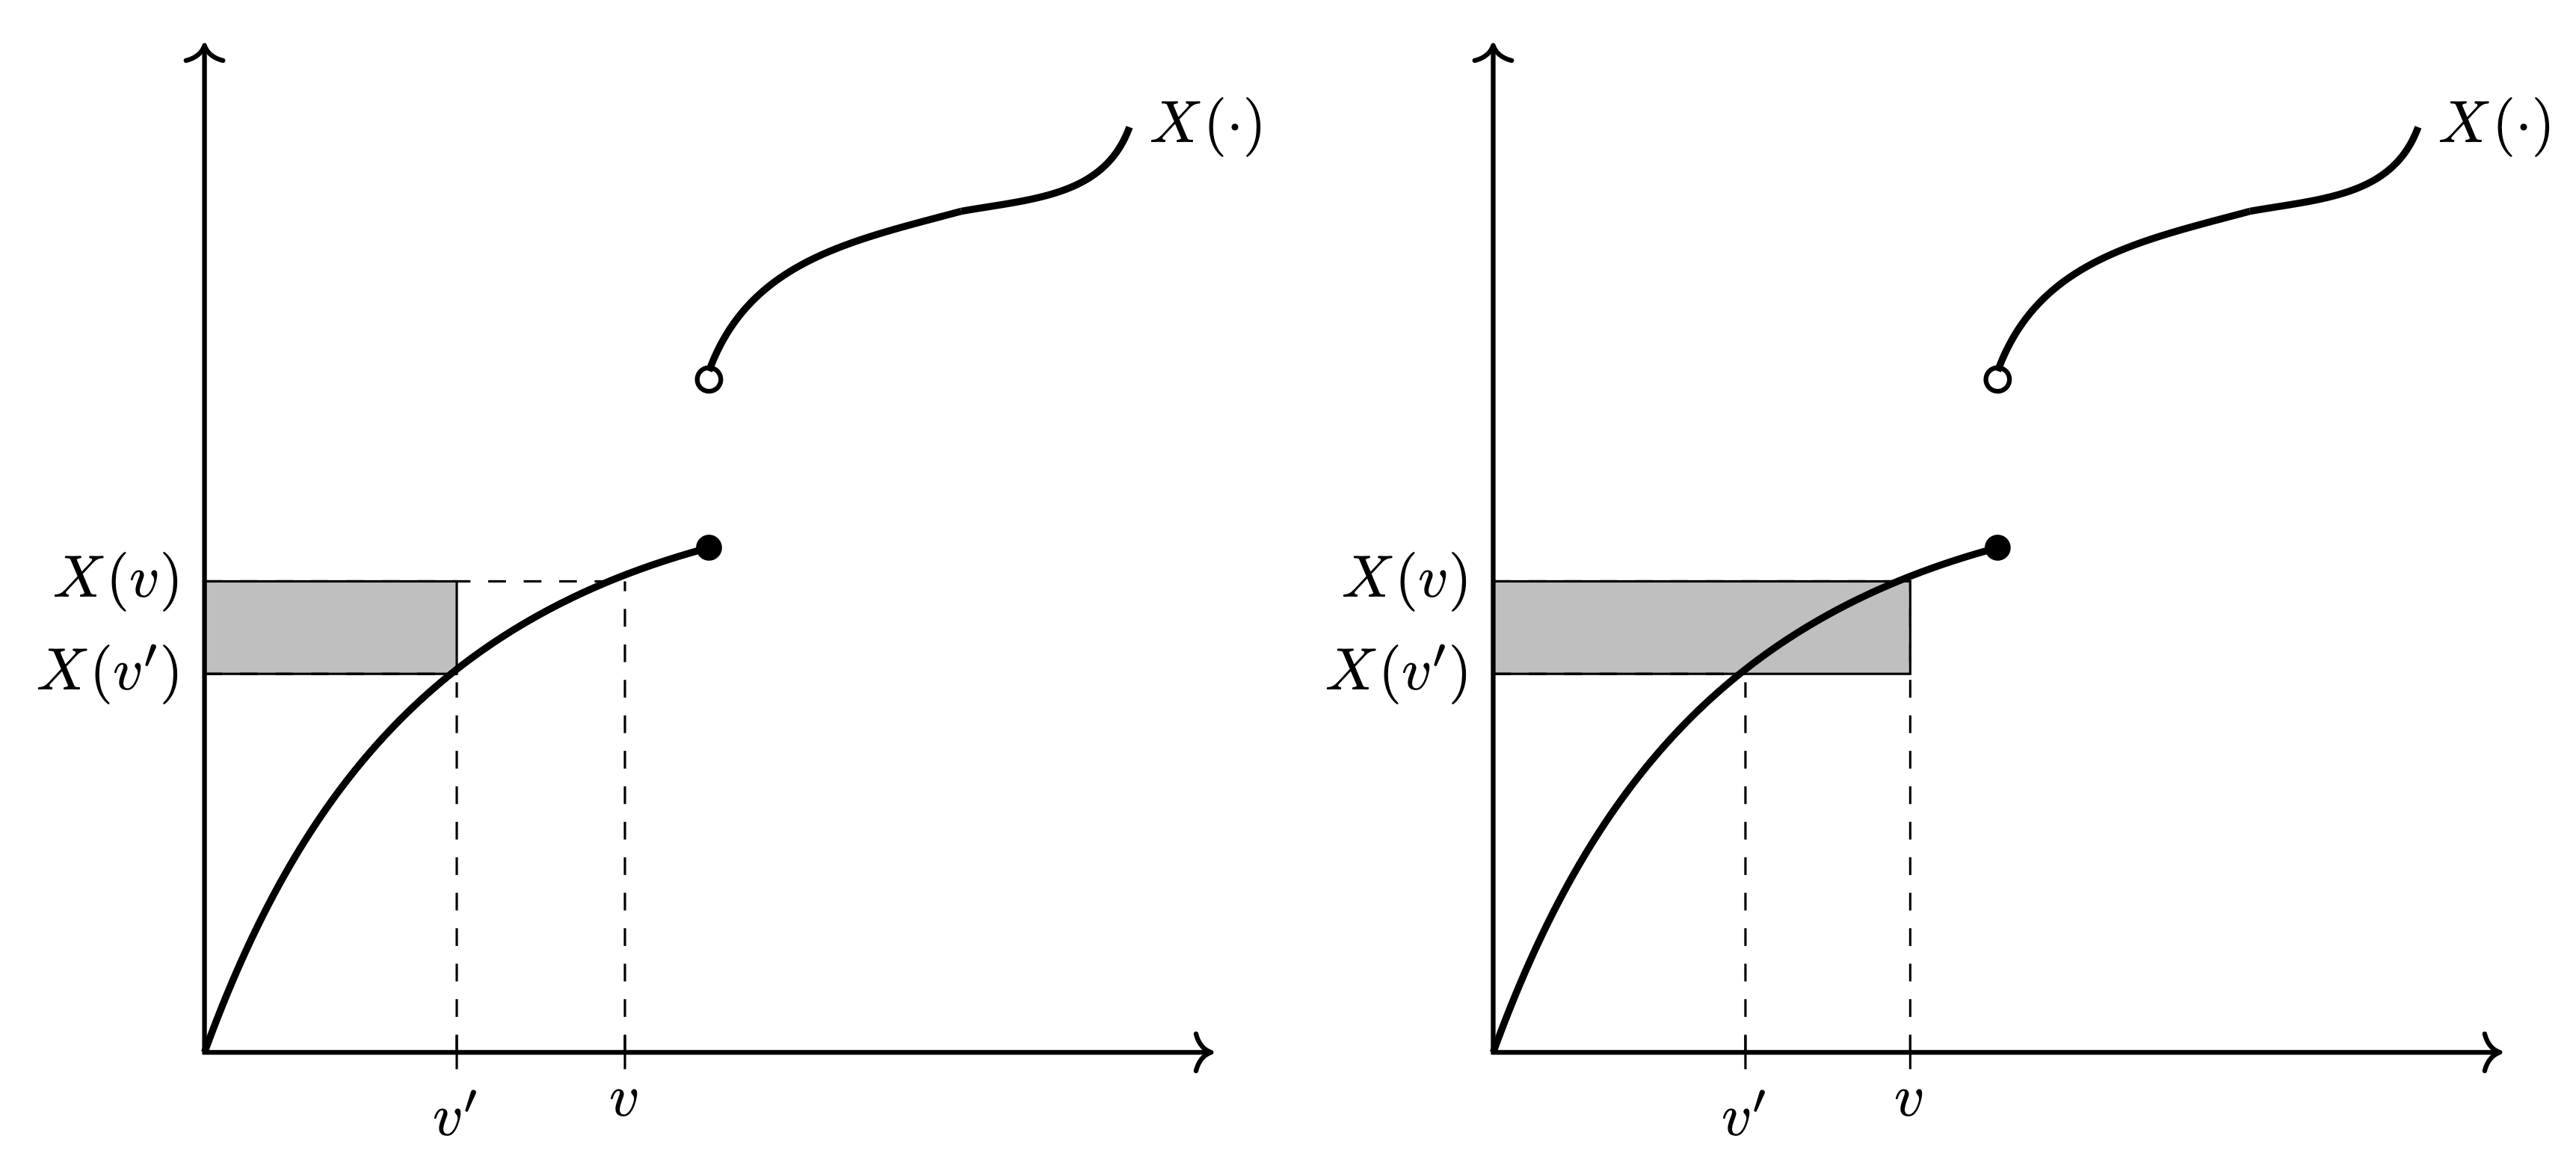
\includegraphics[width=0.78\textwidth]{images/4-20-1}
\fignote{The second approximation to the Riemann integral: summing along values of $X(\cdot)$.}
\end{figure}

\begin{definition}[Individual rationality]
	An auction game $G$ with equilibrium $s$ is individually rational if for each $v$, 
	\boxednote{(Interim) individual rationality is a condition that lies somewhere in between ex-ante and ex-post rationality.}
	\[
		vX(v) - P(v) \ge 0
	.\] 
\end{definition}

We see immediately that $P(0) \le 0$ is required for individual rationality, while result (ii) of Proposition (\ref{4-20-b}) implies $P(0)$ should be as large as possible for revenue-maximization. Hence, among individually rational games, a revenue-maximizing payment schedule must have $P\left(0 \right) = 0$.

\begin{corollary}[A revenue-maximizing auction's payments] \label{4-20-c}
	A revenue-maximizing auction satisfying individual rationality has payment schedule \[
		P(v) = vX(v) - \int_{0}^{v} X(t)dt 
	.\] 
	This payment schedule and $X_i(\cdot)$ being nondecreasing (from Proposition \ref{4-20-b}) are necessary conditions for an auction to be revenue-maximizing.
	Note that we have not yet determined what exactly $X(\cdot)$ is in the revenue-maximizing auction.
\end{corollary}

We have now explained why the first-price, second-price, and all-pay auctions all raise the same expected revenue: they all share $X(v)$ as the probability of $v$ being the highest value. \boxednote{We did \emph{not} show that these auctions are revenue-maximizing. (They aren't!)}So they must share the same payment schedule, and hence expected revenue as well.

\begin{proposition}
	For any $G,G'$ and equilibria $s,s'$ such that $X_G$ and $X_{G'}$ are the same and $P_G(0)=P_{G'}(0)$, the revenue is the same.
\end{proposition}
\begin{proof}
	Immediate from Proposition (\ref{4-20-b}).
\end{proof}

So far, we fixed one agent at a time and derived necessary interim conditions for revenue maximization in an individually rational auction.
We now need to construct an ex-post allocation rule and ex-post payment rule that take the entire value profile $v=\left( v_i \right)_{i \in N}$ as input and generate interim objects satisfying those necessary conditions. Under regularity, the virtual value auction provides such a construction.

\begin{definition}[Regular value distribution, virtual value]
	A distribution with CDF $F$ and density $f$ is regular if the virtual value \[
		c(w) \coloneqq w - \frac{1-F(w)}{f(w)}
	\] is strictly increasing.
\end{definition}

\begin{definition}[Virtual value auction] \label{4-22-4}
	In the virtual value auction, all buyers submit their values for the good. Using $F$, the seller converts these to virtual values. If no virtual value is positive, the seller keeps the good. Otherwise, she gives the good to the agent with the highest value. If there are multiple such agents, then each gets the good with equal probability. Buyers pay the lowest value they could have submitted and still won the auction with, i.e. the second-highest value after excluding duplicates.
\end{definition}

\begin{theorem}[Revenue maximization of the virtual value auction]
	Consider individually rational auctions with a single good and symmetric bidders whose values are drawn iid from a regular distribution $F$. One\footnote{Any revenue-maxizing auction must have $x_i(v_i,v_{-i}) = 0$ for any $i$ where $c(v_i) \le 0$ or $c(v_i) < c(v_j)$ for some $j$.} revenue-maximizing auction has assignment probabilities for each bidder $i$ given by
	\[
		x_i \left( v_i,v_{-i} \right) = \begin{cases}
			0, \quad &c(v_i) \le 0 \text{ or } c(v_i) < c(v_j) \text{ for some }j \\
			\frac{1}{m}, \quad & m \coloneqq \left| \left\{j: v_j = v_i\right\} \right|
		\end{cases}
	.\]
	Moreover, the direct mechanism with this allocation rule and payments
	\[
		p_i(v_i,v_{-i}) = v_ix_i(v_i,v_{-i}) - \int_{0}^{v_i} x_i(t,v_{-i})dt
	\]
	is a revenue-maximizing virtual value auction.
\end{theorem}

\begin{proof}
	Without loss, use a game with $\mathscr{A}_i = \left[ 0,1 \right]$. Fix functions $x: V^{\left| N \right|} \to A$, $p: V^{\left| N \right|} \to \R^{\left| N \right|}$ with $V \coloneqq [0,1]$. Write
	\[
		f_N(v) \coloneqq \prod_{j \in N} f(v_j), \quad
		f_{-i}(v_{-i}) \coloneqq \prod_{j \ne i} f(v_j)
	\]
	for the joint densities of all values and of the values other than $i$'s.

	Define the interim allocations and payments
	\begin{align*}
		X_i(v_i) 
		&= \int_{v_{-i}}^{} x_i\left( v_i, v_{-i} \right)f_{-i}(v_{-i}) dv_{-i} \\
		P_i(v_i)
		&= \int_{v_{-i}}^{} p_i(v_i,v_{-i}) f_{-i}(v_{-i}) dv_{-i}
	.\end{align*}
	We know that $X_i(\cdot)$ is nondecreasing. 

	The seller's problem is to maximize her ex-ante revenue with respect to $p_i$ while selecting compatible $x_i$:
	\begin{align*}
		R
		&=\max \sum\limits_{i \in N}^{}\int_{\left( v_i, v_{-i} \right)}^{}  p_i(v_i,v_{-i}) f_N \left( v_i,v_{-i} \right) d(v_i, v_{-i}) \\
		&= \max \int_{\left( v_i, v_{-i} \right)}^{} \left( \sum\limits_{i \in N}^{} p_i(v_i,v_{-i}) \right)f_N \left( v_i,v_{-i} \right) d(v_i, v_{-i}) \\
		&= \max \sum\limits_{i \in N}^{} \int_{0}^{1} P_i(v_i) f(v_i) dv_i \quad \text{by Corollary (\ref{4-20-c})}\\
		&= \max \sum\limits_{i\in N}^{} \left[
			\int_{0}^{1} v_i X_i(v_i)f(v_i)dv_i
			- \underbrace{\int_{0}^{1} \int_{0}^{v_i} X_i(t)dt f(v_i) dv_i}_{(II_i)}
		\right].
		\intertext{We can work on the second term separately:}
		(II_i)
		&= \int_{0}^{1} f(v_i) \left( \int_{0}^{v_i} X_i(t)dt  \right)dv_i \\
		&=\left. F(z) \int_{0}^{z} X_i(t)dt \right|_{z=0}^{1} - \int_{0}^{1} F(v_i)X_i(v_i) dv_i \\
		&= \int_{0}^{1} X_i(t)dt - \int_{0}^{1} F(v_i) X_i(v_i) dv_i \\
		&= \int_{0}^{1} \left( 1- F(v_i) \right)X_i(v_i)dv_i 
		\intertext{Substituting $(II_i)$ back in,}
		R 
		&= \max \sum\limits_{i \in N}^{} \int_0^1 \left( \overbrace{v_i - \frac{1-F(v_i)}{f(v_i)}}^{\mathclap{\smash{\text{virtual value}}}} \right) X_i (v_i) f(v_i) dv_i \\
		&= \max \int_{\left( v_i,v_{-i} \right)}^{} \sum\limits_{i \in N}^{} \left(\underbrace{ v_i - \frac{1-F(v_i)}{f(v_i)}}_{\mathclap{\smash{\coloneqq c(v_i)}}} \right) x_i(v_i, v_{-i}) f_N(v_i, v_{-i}) dv
	.\end{align*}
	\boxednote[-32\baselineskip]{In this step, we relate the seller's ex-ante expected revenue to an individual's interim expected payment. This is not just because we have the identity for the interim payment from Corollary (\ref{4-20-c}), but also because interim objects are what agents have strategies over.}
	\boxednote[-9\baselineskip]{This line tells us that for a given value profile of agent $i$, the expected amount the seller earns from $i$ is the virtual value $c_i$ times the interim assignment probability, which does not condition on others' values.}
	\boxednote[-4\baselineskip]{This line tells us the expected amount the seller earns from $i$ is exactly the virtual value $c_i$ times the probability that $i$ gets the good under a given value profile of $(v_1,\ldots,v_{\left| N \right|})$.}
	With a fixed value profile $v$, then $R$ is maximized by setting
	\begin{equation}
		x_i (v_i, v_{-i}) = 
		\begin{cases}
			0, \quad & c(v_i) \le 0 \text{ or } c(v_i) < c(v_j)\text{ for $j \ne i$} \\
			\frac{1}{m}, \quad &\text{otherwise, where } m\coloneqq \left| \left\{j: v_j = \max_i \left\{v_i\right\}\right\} \right|
		\end{cases} \label{4-22-2}
	.\end{equation}
	We have derived a candidate function for the win probabilities. If an auction is revenue-maximizing, then it must use these ex-post assignment probabilities.\footnote{At least, it must have zero assignment probability for agents with negative virtual values or virtual values that are not the highest.}

	Recall from Corollary (\ref{4-20-c}) that there are two more necessary conditions for an auction to be revenue-maximizing and individually rational:
	\begin{enumerate}[label = (\roman*)]
		\item The interim win probabilities $X_i$ are nondecreasing, and
		\item The interim payments must satisfy
			\begin{equation}
				P_i(v_i) = v_i X_i(v_i) - \int_{0}^{v_i} X_i(t)dt 
				 \label{4-22-1}
			.\end{equation}
	\end{enumerate}
	We check the first:
	because $F$ is regular, we know that $X_i(\cdot)$ is nondecreasing; a higher value leads to a higher virtual value, which $X_i(\cdot)$ is increasing in. In particular, the good is allocated to an agent with the highest value.

	Now we need to determine the payments in a way that will satisfy the second condition.
	We can easily get payments that satisfy the interim payments' characterizations by putting \[
		p_i(v_i,v_{-i}) \coloneqq v_ix_i(v_i,v_{-i}) - \int_{0}^{v_i}  x_i(t,v_{-i})dt
	,\] as integrating both sides recovers Equation (\ref{4-22-1}).

	The candidate optimum assignment probability in Equation (\ref{4-22-2}) is currently written in terms of the virtual values; let's rewrite it in terms of the actual values. Let $\underline{v}$ be the unique\boxednote{We know that $\underline{v}$ must be unique because we assumed $F$ is regular, and so $c$ is strictly increasing.} value such that $c(\underline{v}) = 0$, or $0$ otherwise. Put $s \coloneqq\max \left\{\underline{v}, v_j\right\}_{j \ne i}$.

	We have three cases.
	\begin{description}
		\item[Case 1]: If $v_i < s$, then agent $i$ pays \[
			v_i \cdot 0 - \int_{0}^{v_i} \underbrace{x_i(t,v_{-i})}_{=0}dt = 0
		.\]
		\item[Case 2]: If $v_i > s $, then agent $i$ pays \[
			v_i \cdot 1 - \int_{0}^{v_i} x_i(t,v_{-i})dt = v_i - v_i + s = \max \left\{\underline{v}, v_j\right\}_{j\ne i}
		.\]
		\boxednote{We see that if there is a single winner, as in Case 2, then she pays according to a second-price auction, unless the second-highest value is below the reserve value, in which case she pays the seller's reserve value.}
		\item[Case 3]: If $v_i = s \ne \underline{v}$ and $m$ people have the highest value, then agent $i$ pays \[
			v_i \cdot \frac{1}{m} - \underbrace{\int_{0}^{v_i} x_i(t,v_{-i}) dt}_{=0} = \frac{v_i}{m}
		.\]
	\end{description}
	
	The ex-post assignment probabilities $x_i$ were the only candidates for an optimal auction, while the payments $p_i$ just needed to satisfy the condition on the interim payments $P_i$ given by Corollary (\ref{4-20-c}).
	It is simple to show that the auction defined by $(x_i,p_i)_{i \in N}$ is incentive-compatible, and thus constitutes an equilibrium (in which everyone reports their true values).
\end{proof}

\begin{remark}
	There are several nice properties of our solution:
	\begin{enumerate}[label = (\roman*)]
		\item We set out to find a Bayes--Nash equilibrium, but got an auction that also is implementable in dominant strategies. This is a subclass of Bayes--Nash equilibria in which universal truth telling is the specific equilibrium.
		\item We just wanted interim individual rationality, but ended with ex-post individual rationality as well.
		\item If $\left| N \right| = 1$, then there is a posted price at $\underline{v}$, which aligns exactly with our finding from Proposition (\ref{4-22-3}).
	\end{enumerate}
\end{remark}

\section{Multiple Goods and a Single Buyer}

Now we consider when the seller has two goods to sell and there is a single buyer with values $v^1$ and $v^2$. If the buyer has probability $x^1$ of getting good 1 and probability $x^2$ of getting good 2 with payment $p$, then the interim expected utility\boxednote{This structure on the expected utility imposes that the utility function is separable in the two goods.} is defined to be \[
	v^1x^1 + v^2x^2 - p
.\] Assume $v^1 \sim F^{1}$ and $v^2 \sim F^2$ independently.

\begin{proposition}
	In a two-good, single buyer auction with independent value distributions $F^1, F^2 \sim \operatorname{Unif}(0,1)$, the optimal mechanism is one in which the buyer has the options to:
	\begin{enumerate}[label = (\roman*)]
		\item Buy either good at price $\frac{3}{4}$, or
		\item Buy both goods at price $\frac{4-\sqrt{2} }{3}$.
	\end{enumerate}
\end{proposition}
\begin{proof}
	We omit the proof.
\end{proof}

More generally, a mechanism can offer a menu of the form \[
	\left\{\left( z^1, z^2, z^{12} \right),p\right\}
,\] where $p$ is the payment required for the agent to receive assignment probabilities $z^1,z^2,z^{12}$. 
\begin{proposition}
	If both $F^1$ and $F^2$ are Beta distributions, the optimal mechanism offers an uncountably large menu.
\end{proposition}

For intuition on why bundling the two goods together is more profitable for the seller than keeping them separate, we know that if the goods were to be sold individually, we would have two posted price auctions at price \[
	p^\star = \frac{1-F(p^\star)}{f(p^\star)} = \frac{1}{2}
.\] 
Then the bundle purchased is \[
	\begin{cases}
		\O, \quad &v_1, v_2 < \frac{1}{2} \\
		\left\{1\right\}, \quad & v_2< \frac{1}{2} \le v_1 \\
		\left\{2\right\}, \quad & v_1 < \frac{1}{2} \le v_2 \\
		\left\{1,2\right\}, \quad &\frac{1}{2} \le v_1,v_2
	\end{cases}
.\] 
When bundling with the option to buy $\left\{1,2\right\}$ at discount of $\delta$ (so the price of the bundle is $p \coloneqq 1-\delta$), an agent who buys the bundle will satisfy:
\begin{enumerate}[label = (\roman*)]
	\item $v_1 + v_2 > 1-\delta$
	\item $v_1 + v_2 - p > v_1 - \frac{1}{2} \iff v_2 > p - \frac{1}{2}$
	\item $v_1 + v_2 - p > v_2- \frac{1}{2} \iff v_1 > p-\frac{1}{2}$.
\end{enumerate}

These define regions in the joint value distribution displayed below.

\begin{figure}[htpb]
\centering
\caption{The effect of introducting a bundle at price $p \coloneqq 1-\delta$ on revenue.}
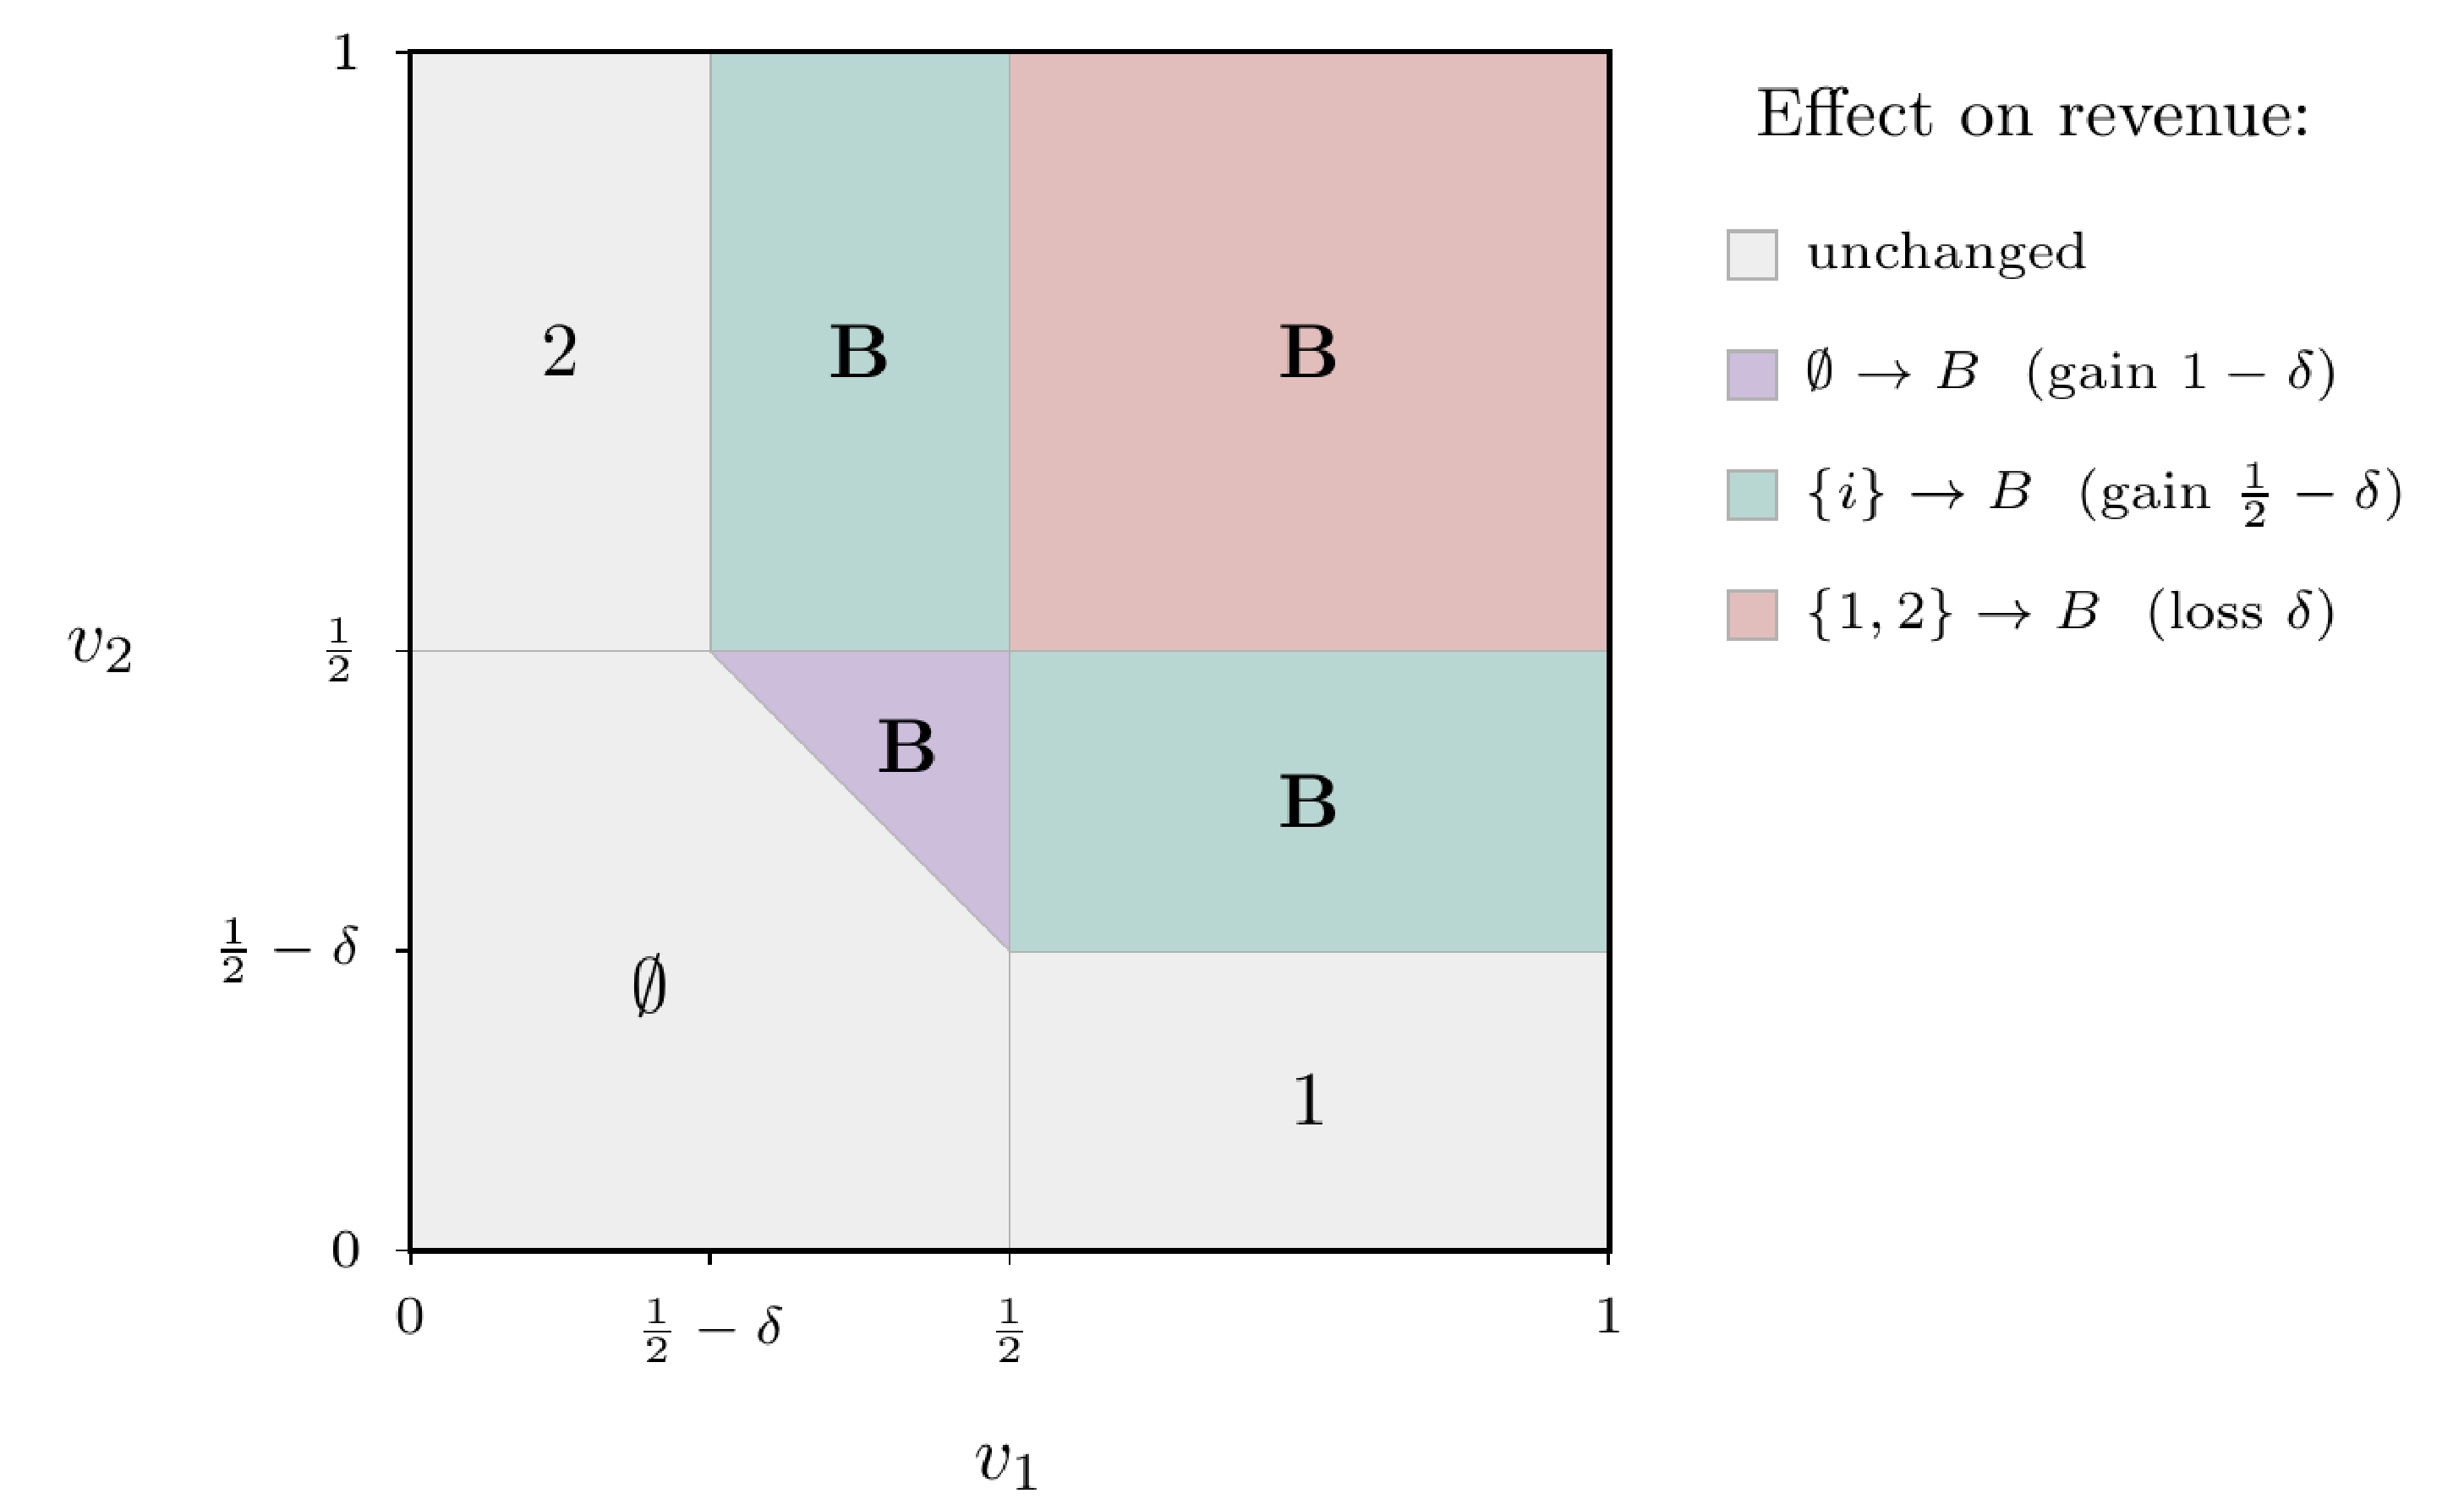
\includegraphics[width=0.78\textwidth]{images/4-29-1}
\fignote{
The original region of both-object-buyers was the red square, while we have now added the other shaded regions.
}
\end{figure}

The total change in revenue from the green regions is $2\left( \delta \frac{1}{2} \right)\left( 1- \delta - \frac{1}{2} \right) = \delta (\frac{1}{2} - \delta)$. The change from the purple region is $\frac{1}{2} \delta^2(1-\delta)$, and the change from the red region is $-\frac{1}{4}\delta$.
Hence, the total change in revenue is \[
	\Delta = \delta( \frac{1}{2} - \delta) + \frac{\delta^2}{2}(1-\delta) - \frac{1}{4}\delta = \frac{\delta}{2} - \delta^2 + \frac{\delta^2}{2} - \frac{\delta^3}{2} - \frac{1}{4}\delta
,\] which is close to $\frac{\delta}{4}$ when $\delta$ is close to zero. Note that when $\delta = 0$, we recover the individual auction case, but $\left.\partial_\delta \Delta\right|_{\delta = 0} \Delta > 0$, so it would be profitable to bundle at a discount.
